
%(BEGIN_QUESTION)
% Copyright 2010, Tony R. Kuphaldt, released under the Creative Commons Attribution License (v 1.0)
% This means you may do almost anything with this work of mine, so long as you give me proper credit

Beregn spenningsfallet over RTD-elementet i denne kretsen, utgangsspenningen fra operasjonsforsterkeren, og temperaturmålefeilen basert på avviket mellom disse to spenningene:

$$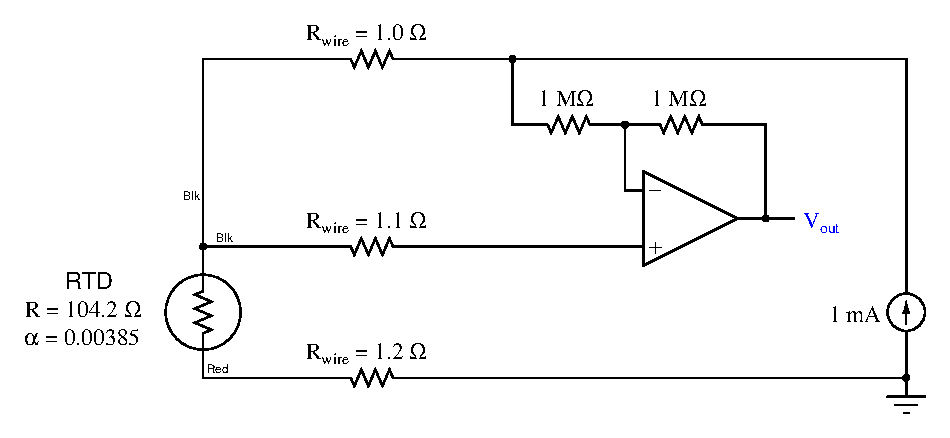
\includegraphics[width=15.5cm]{i00041x01.eps}$$

$V_{RTD}$ = \underbar{\hskip 50pt}

\vskip 10pt

$V_{out}$ = \underbar{\hskip 50pt}

\vskip 10pt

Temp.-feil = \underbar{\hskip 50pt}

\vskip 20pt

Merk: RTD-en i denne kretsen er en "100 ohm" platinasensor, men den faktiske motstanden ved denne temperaturen er 104.2 $\Omega$.

\vfil 

Merk: for å forenkle analysen kan du anta at strømmen gjennom 1 M$\Omega$-motstandene er null.  Den faktiske strømmen er så liten at den kan neglisjeres.

\underbar{file i00041}
\eject
%(END_QUESTION)





%(BEGIN_ANSWER)

Dette er et vurdert spørsmål -- ingen svar eller hint gis!

%(END_ANSWER)





%(BEGIN_NOTES)

Du vil {\it ikke} kunne løse spenninger og strømmer i denne kretsen ved å bruke memorerte forsterkerformler for opamp-kretser, siden dette ikke er en vanlig forsterkerkrets.  I stedet må du analysere den fra "første prinsipper" (f.eks. Kirchhoffs spenningslov, Ohms lov, forenklede antakelser for opamp-kretser med negativ tilbakekobling, osv.).

\vskip 10pt

Når det gjelder opamp-kretser med negativ tilbakekobling, bruk alltid disse forenklede antakelsene for å gjøre analysen håndterbar:

\begin{itemize}
\item{} Negativ tilbakekobling vil tvinge utgangsspenningen til den verdien som er nødvendig for å holde differensial-inngangsspenningen lik null.
\item{} Inngangsterminalene på opampen trekker neglisjerbar strøm.
\end{itemize}

$$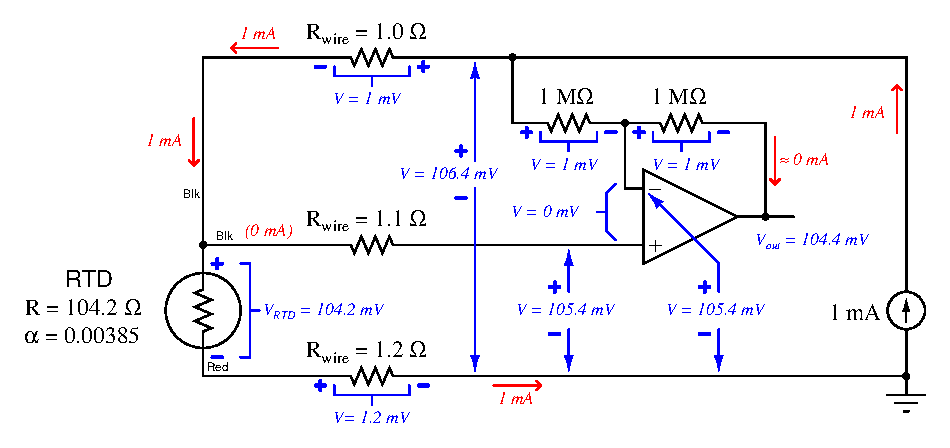
\includegraphics[width=15.5cm]{i00041x02.eps}$$

Som du kan se her, faller 104.2 mV over RTD-en mens opampen gir 104.4 mV, en feil på 0.2 mV.  Motstandsfeilen som tilsvarer 0.2 mV (ved en eksitasjonsstrøm på 1 mA) er 0.2 ohm.  Gitt en basisresistans på 100 ohm og en alpha-koeffisient på 0.00385, tilsvarer denne motstandsfeilen en temperaturfeil på 0.519 $^{o}$C eller 0.935 $^{o}$F.


%INDEX% Measurement, temperature: RTD

%(END_NOTES)
